\documentclass[final]{IEEEtran}

\usepackage[utf8]{inputenc}
\usepackage[noadjust]{cite}
\ifCLASSINFOpdf
  \usepackage[pdftex]{graphicx}
\else
  \usepackage[dvips]{graphicx}
\fi
\usepackage{amsmath}
\usepackage{array}
\usepackage{url}
\usepackage{paralist}
\usepackage{enumitem}

\begin{document}
\title{User Data Analysis with Data Mining}

\author{\IEEEauthorblockN{Péter Ivanics}
\IEEEauthorblockA{Department of Computer Science \\
University of Helsinki \\
Email: peter.ivanics@helsinki.fi \\
\url{http://pivanics.users.cs.helsinki.fi/portfolio/}}}

\maketitle

\begin{abstract}
%<Context>
Many software businesses collect enormous amount of data generated by end-users. End-user data incorporates essential information about how users interact with the system of discussion as well as information about the users themselves. Such digital footprints can explain the preferences of users, what kind of content they like, how frequent their activity in the platform is, in what ways they interact with the system and eachother.

%<Objectives>
The goal of this research is to study the potential use of user data in business and research environments with the application of Data Mining methods. Since there is no common understanding on its concept, initially user data is defined. Secondly, it is studied how user data is utilized in related studies and what kind of results can be derived from such dataset. For example, user data of social media sites can reveal what kind of feedback is received from the engaged audience in terms of like activities and comments on the uploaded content. Thirdly, the demographic characteristics of users are put in studied in relation to the content which engages them online.

%<Methods>
The findings are retrieved by reviewing relevant literature. The sources include scientific journals, articles as well as books related to the topic of this study. 

%<Results>
The research papers in the field show various ways how user data can be used. By the application of machine learning, image processing and natural language processing techniques, several researchers have successfully extracted novel results from user data. The reviewed literature clearly suggests the relevance of studying user data.

\end{abstract}

\begin{IEEEkeywords}
  user data, data mining, user behavior
\end{IEEEkeywords}

\section{Introduction}
% context, setting - B2C business gathers a lot of data
Many software businesses collect enormous amount of data generated by end-users \cite{chinesemobilebankingusers, bigdatamanagementrevolution, inmon2007tapping}. End-user data incorporates essential information about how users interact with the system of discussion as well as tells a lot about the users themselves \cite{jang2015noreciprocity, hu2014we, jang2016teensengagemorewithfewerphotos, han2016teensarefrommars, socialdiversityongithub}. For instance, such data can explain the preferences of users, what kind of content they like, how they interact with the system and eachother or how frequently they use the software that has generated the data \cite{youyou2015computer}\cite{ottoni2013ladies}.

% what is the challenge?
 Depending on the portfolio of the business, analysis of end-user data can reveal various interesting findings. For instance, in banking industry Big Data tools are often used to analyze demographic characteristics to maintain and establish new client relationships \cite{chinesemobilebankingusers}\cite{bigdatamanagementrevolution}. Extracting the information from the data is challenging: most businesses are to collect more data than what is humanly possible to process and to analyze \cite{inmon2007tapping}\cite{wegener2010integrating}. As a result, significant part of the knowledge might remain hidden and hence business-critical information remains unseen \cite{chinesemobilebankingusers}\cite{inmon2007tapping}\cite{wegener2010integrating}\cite{introtodatamining}. The computational methods of today's world enable us not only to achieve previously impossible tasks, but also to create tools that may outperform humans \cite{youyou2015computer}. Accordingly, there is a growing need for all businesses to introduce data analysis processes in their daily activities with the aim of understanding users and data generated by them better.

 % how do mobile devices have an impact on the amount of data? 
 With the continuous growth of mobile devices in numbers, the amount of data has increased significantly. Due to the wide availability and commonness of smartphones and tablets, anybody can easily generate rich location, media or textual data \cite{jang2016teensengagemorewithfewerphotos}. Complementary to the popularity of mobile devices, social media sites have grown a lot in the past years \cite{hu2014we}\cite{ottoni2013ladies}\cite{bakhshi2014faces}, allowing users rich ways of interaction. Due to the combination of these two trends, users leave digital footprints as location, media, numerical or textual data in numerous places around the Internet \cite{youyou2015computer}. People often express their opinion by sharing, liking or commenting on data over social networks. Study shows, that algorithms can predict users' personality traits using such data more reliably than other humans would do \cite{youyou2015computer}. These facts further increase the call for research in the field of mobile and user data analysis, because it can help researchers to understand the society, human behavior, preferences and public opinions better.

 % what is the potential in analyzing user data? why is it important not only to collect but also analyze data?
 Data analysis tools and methods already exist to facilitate processing user data. However, these applications often not utilized, because companies rather focus on developing their service package than understanding the information gathered in the past \cite{bigdatamanagementrevolution}\cite{inmon2007tapping}. Therefore, Knowledge Discovery in Databases is important and is essential part of Business Intelligence applications as well \cite{bigdatamanagementrevolution}\cite{zarsky2002mine}.

 % what is the goal? what is this thesis about?
 The goal of this research is to study understand the potential use of user data in business and research environments in the present time. The study looks into related researches to argue for the relevance of Data Mining methods in the area. The research aims to study how content on the Internet is observed by the users, who access the content. Secondly, it is studied what kind of feedback is received from the engaged audience in terms of like activities and comments to the provided content. Thirdly, the tendencies among the demographic characteristics between users are studied in relation to the content which gets them engaged online. 

The motivation behind conducting this research are the stimulating challenges about user data and the wide possibilities of the information that it contains. Studying this field are interesting not only for computer scientists but from the point of view of human behavior research. This paper aims to seek answers to the following research questions by discussing relevant literature in the topic: 

\pagebreak

\setdefaultleftmargin{40pt}{}{}{}{}{}
\begin{enumerate}[label=RQ\arabic*:]
	\item How is user data understood in previous research?
	\item How data mining methods are utilized for user data analysis in scientific researches?
\end{enumerate}

% how is the rest of this paper structured? 
The rest of this paper is organized as follows. The following section presents the selected research methods for this literature review. Section III introduces the concept of user data and explains, how is it understood and used in related studies. Section IV explains the related studies where user data is studied and presents the most commonly used techniques for its analysis. Section V discusses the previously presented results by analyzing and comparing the findings of other researchers in the field. Finally, Section IV concludes the research and pinpoints directions for further studies. 

\section{Research methods}
The foundations of the theoretical basis are retrieved by reviewing relevant literature. The sources include scientific journals, articles as well as books related to the topic of this study. The two former sources are retrieved through three online digital libraries: the ACM digital library, IEEE Xplore and Google Scholar. 

After finding the first papers, the snowballing technique was used to retrieve further papers in the field. Various keywords were used to obtain related literature in the research area. Keywords included, but were not limited to "data mining", "social media", "user data", "user behavior", "demographic characteristics" and "digital footprints". The retrieved papers are then critically analyzed and the most interesting points from and across the studies are summarized in this short paper. The emphasis is placed on the research goals towards which other studies utilize demographic and user data as well as the computational methods, that were chosen by other researchers. 

% \section{The concept of user data}
\section{Terminology}
% what is user data? what does it include or exclude?
Despite the fact the term user behavior is widely studied, researchers claim that its concept is used rather ambiguously \cite{waheed2017investigation}. Therefore, a formulation is made on its concept to establish the ground for this literature review. The term user data in this study covers two major kind of data that is related to users. On one hand it covers data, which is willingly uploaded and generated by users, on the other hand, it consists of data which generated through interactions while using software solutions (typically online). Figure \ref{user_data_venn} demonstrates how user data is understood in this study.

% demographic characteristics
The first part of user data typically consists of the demographic characteristics of the users and the content which they have generated \cite{han2016teensarefrommars}. Traditionally demographic data is often collected via surveys and questionnaires by researchers. This kind of data often can be found on social media profiles where social demographic information, such as gender, age and nationality are shared. As a result, this kind of data can be obtained relatively easily in vast amount, if users as eager to share with the software service provider.

% digital footprints
Secondly, data gathered during the usage of a software is an important source of information for scientific studies. Researchers use the term digital footprint \cite{youyou2015computer} to describe this kind of data, which composes the second type of user data in this research. Such digital footprints can vary a lot depending on the software of discussion, but typically consists of like activities, user comments, photos, posts on social media, ratings in movie databases or browsing history and usage patterns for web browsers. 

\begin{figure}[h] 
  \begin{center}
    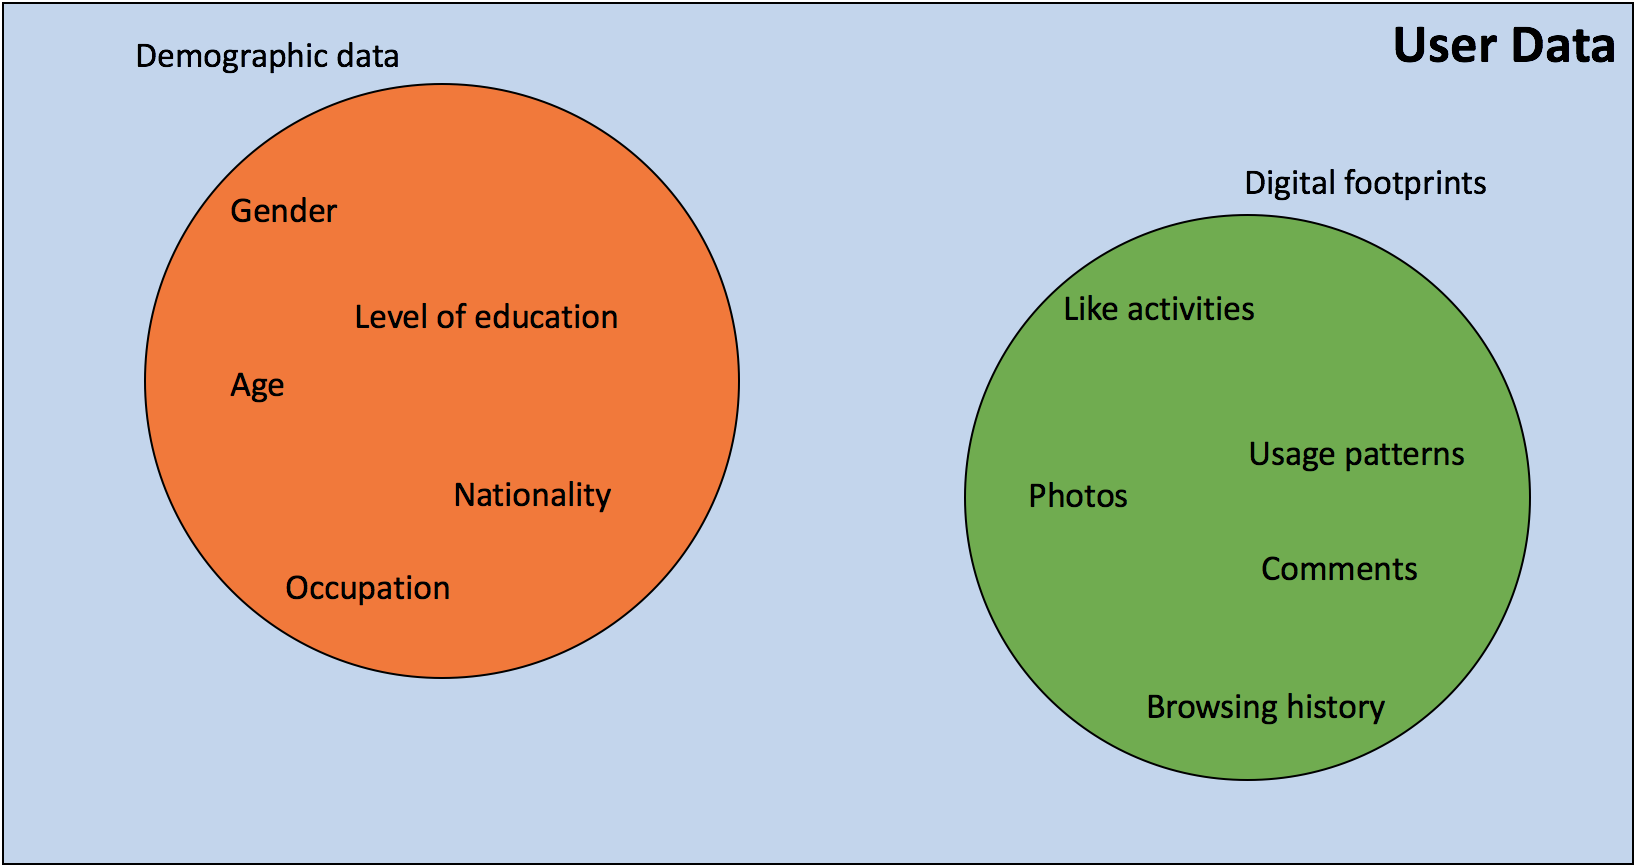
\includegraphics[width=3in]{Images/user_data_venn.png}
    \caption{User data in this research is the combination of users' demographical characteristics and digital footprints.}
    \label{user_data_venn}
  \end{center}
\end{figure}

\section{User data analysis}
\subsection{Related research}
Previous research have proven the relevance of statistical analysis on Big Data, such as like activities \cite{jang2015noreciprocity}\cite{jang2016teensengagemorewithfewerphotos}\cite{ottoni2013ladies}\cite{guy2016whatsyourorganizationlike}\cite{jang2015no}, user comments \cite{jang2016teensengagemorewithfewerphotos}, tags under images \cite{jang2016teensengagemorewithfewerphotos}, image content \cite{hu2014we}\cite{bakhshi2014faces} and movie ratings \cite{saraee2004data}\cite{kabinsingha2012movie} by revealing interesting findings about user behavior. Moreover, as service providers often get access to user demographics-related data through social network sites in the present time, new possibilities become available to seek correlation between user segments. 

% explain that these are often not studied together but rather separately 
The concepts of demographical characteristics and digital footprints are widely studied in the research field, but often only separately, focused on one certain area. Demographic characteristics play a role in analyzing user adoption and behavior, for instance in the banking industry. The study conducted by Wang and Petrounias \cite{chinesemobilebankingusers} reveals that mobile banking in China is more popular among middle-aged males, while the younger generation has not adopted to the new trends yet. By utilizing Big Data analytics the group of citizens and products for the upcoming marketing campaigns were revealed \cite{chinesemobilebankingusers}, which greatly enhances the marketing activities of financial organizations. Social diversity was also studied by other researchers in the context of software development growth \cite{socialdiversityongithub}. In their study, Aué et al. \cite{socialdiversityongithub} have clearly identified correlation between the success of open source projects and the contributors' gender and cultural diversity by utilizing well chosen statistical methods. 

% what kind of results were derived in the past from end-user data analysis? 
Movie databases often contain user reviews on movies, actors and producers of all sort. Such databases are open and are available for the public, and therefore the amount of data has grown huge over the past years. Unsurprisingly, databases like the Internet Movie Database (IMDB) has drawn the interest of researchers \cite{saraee2004data}\cite{kabinsingha2012movie}\cite{sumathi2013performance}. The successful application of statistical methods and data mining techniques have revealed interesting findings. Studies have proven that larger budget for movies does not necessarily result in good ratings by the public, while actors have higher impact on the opinion of the audience \cite{saraee2004data}. On top of deriving such conclusions, machine learning techniques are emerging to predict future movie rating data, based on prior reviews of users \cite{saraee2004data} or the analysis of genre and other attributes of movies \cite{kabinsingha2012movie}.

% how do researches on social media website data see the user data analysis?  
Social Networking Sites (SNSs) are another trending source in discovering the secrets of user data as the number of scientific publications in the topic has increased significantly in the recent years \cite{waheed2017investigation}. Various researches have applied advanced data mining techniques on Instagram data \cite{jang2015noreciprocity}\cite{bakhshi2014faces}\cite{hu2014we}\cite{jang2016teensengagemorewithfewerphotos}\cite{han2016teensarefrommars}, more specifically on the tags and comments that are attached to the images. Similarly, like activities and user-generated content is studied by the scientists. It is revealed, that Instagram users can be divided into two groups based on their activities: specialists, who publish and seek content around a certain topic of interest; and generalists, who are interested in all kinds of genres in the social media site \cite{jang2015noreciprocity}. Data mining techniques also allowed researchers to conclude, that the teenager users of Instagram tend to be more active, faster to react and more open to communicate with other users on social media \cite{jang2016teensengagemorewithfewerphotos}\cite{han2016teensarefrommars}. Furthermore, it was discovered that media content with human faces are more engaging than other type of media \cite{bakhshi2014faces}. Finally, rich social media data allowed researchers to analyze behavior and user preferences among genders, age groups and locations \cite{farseev2015harvestingmultiplesources}.

Like activities performed on social media are widely studied concept \cite{bakhshi2014faces}\cite{jang2015noreciprocity, jang2016teensengagemorewithfewerphotos}\cite{ottoni2013ladies}. Comments, hashtags and content that is generated by users are also widely studied \cite{bakhshi2014faces}\cite{jang2016teensengagemorewithfewerphotos}\cite{hu2014we}\cite{bakhshi2014faces} and also contribute to this kind of data in this study. However, little research has been conducted in the field on how these usage patterns can be projected onto demographical data, which can greatly contribute to understand user behavior of certain target groups. 

% where is all this research coming from?
Interestingly, most of the SNS-related studies are conducted in the United States of America and Asia \cite{waheed2017investigation}. Only a few studies were conducted in the European region, which allows to conclude that there is a great interest and development possibility in the area. However it is important to highlight, that due to the wide popularity of the international social networks (such as Facebook, Instagram or Pintrest), some part of the data may be derived from users in the European continent. It was also pointed out that some researches focus on sites, that are specific to a particular region or country \cite{waheed2017investigation}, which means the findings are strongly related to the cultural environment of the user base. 

% facebook reactions
Recently Facebook has introduced reactions among their features. Through reactions, users can not only "like" content, but also express other emotions, such as love, joy, amazement, anger or sadness \cite{shouldfacebookusereactions}\cite{howarenewspublishersreactingonfacebook}. This way users' emotional feelings about the content can be collected easily and efficiently. Shortly after its release, it was identified that the new feature is very popular and generally engages a wider audience than previous likes and comments \cite{shouldfacebookusereactions}. Study also shows, that reactions are a great way for publishers to get a feedback on the public's opinion \cite{howarenewspublishersreactingonfacebook}. On top of that, reactions offer an easy way for content providers to organize a by assigning one of the available reactions to the participants and asking the users to react on the content with their favorite's reaction \cite{shouldfacebookusereactions}. The limitation on such polls is that users have the possibility to choose only one of the reactions and hence only one of the participants as their answer to the voting. Despite its wide availability and potential, there was no comprehensive study conducted in this area until this date.

% what does user data analysis reveal in a corporate social media environment? [refer to \cite{guy2016whatsyourorganizationlike}]
Social media platforms in enterprise environment are studied similarly to regular social networks \cite{guy2016whatsyourorganizationlike}. Despite the fact that the two types of social media platforms share many features, analysis performed in enterprise environment can provide great insights about how employees interact and cooperate. Among many other findings, studies have shown that blogs posts in an enterprise social media site tend to be more engaging and contribute to form communities inside the organization \cite{guy2016whatsyourorganizationlike}. Such insights are essential for higher management, because it can be used for instance to identify departments that tend to be less interactive or engaged.  

\subsection{Tools and methods}
Various methods were utilized in previous research to conclude the findings above. The major categories of the techniques and their purposes are explained in the paragraphs to follow. Table \ref{table_of_techniques} below lists the same findings.

% what methods are utilized? 
  % multiple data sources
   The combination of multiple data sources containing users' demographic data, such as Facebook, Instagram, Pintrest or other social media services, is a common practice in researches \cite{farseev2015harvestingmultiplesources}\cite{ottoni2013ladies}. Researchers have managed to perform complete demographic profiling and concluded that the integration of multiple data sources is indeed a great method of enhancing performance on user data analysis \cite{farseev2015harvestingmultiplesources}. 
  
  Utilizing additional tools, existing datasets can be further enhanced for data analysis purposes. A great specimen for this is computer vision, which is used in numerous studies to identify content of photos \cite{hu2014we}\cite{farseev2015harvestingmultiplesources}. In two of the reviewed papers \cite{han2016teensarefrommars}\cite{bakhshi2014faces}, computer vision techniques are utilized to identify faces on and predict ages of people from photos uploaded to social media sites. Through these researches, computer vision was proven to be a powerful tool to facilitate the knowledge by providing researchers further data for their studies. 

  % text processing techniques
  Text processing techniques are potentially the most common way to discover the insights of user data. The Linguistic Inquiry and Word Count (LIWC) and Latent Dirichlet Allocation (LDA) methods are used by researchers \cite{ottoni2013ladies}\cite{farseev2015harvestingmultiplesources, jang2016teensengagemorewithfewerphotos} for extracting linguistic features of text. In their study, Jang et al use this technique to identify keywords and perform topic modelling based on users' comments and hashtags on Instagram \cite{jang2016teensengagemorewithfewerphotos}. Topic modelling was also applied for analyzing genres of movies by their title and description \cite{kabinsingha2012movie}. Applying natural language processing techniques also allowed researchers to infer age and gender of users \cite{han2016teensarefrommars} who have commented on content on Instagram. Utilizing these methods greatly contribute to the understanding of data gathered, which can lead to richer analysis and pattern recognition on the dataset at hand. 

  % supervised ML techniques
  Supervised machine learning appears to be a popular technique for prediction tasks performed on user data. For example, decision trees are utilized as prediction tools for the purposes of identifying audience of mobile banking software in China \cite{chinesemobilebankingusers}. Decision trees were also successfully used for movie rating prediction \cite{saraee2004data} and classification of movies \cite{kabinsingha2012movie}. Bayesian networks in the same study \cite{kabinsingha2012movie} are also investigated and are found as the most suitable method for predictions in the field of movie rating prediction. Ensemble Modeling, which is another supervised learning method, is successfully used for user profile learning on social media sites \cite{farseev2015harvestingmultiplesources}. Similarly, Support Vector Machines and Logistic Regression was utilized for predicting age group of users based on their social media activities \cite{han2016teensarefrommars}. Last, but not least Negative Binomial Regression is put in use to model like activities in researches \cite{jang2015no, bakhshi2014faces}.

  % unsupervised learning - less popular but still possible
  Unsupervised machine learning techniques are also present in the literature, however on a smaller scale. As an example, clustering is used by Saraee White and Eccleston \cite{saraee2004data} for detecting relationships between the ratings given on a movie and the year it was published. The study by Hu et al. \cite{hu2014we} uses the k-means algorithm was used successfully to create five clusters of Instagram users based on the type of content they have uploaded to Instagram. These results share similarities with another study by Jang et al. \cite{jang2015no}, where generalist and specialist groups were identified based on their like activities based on natural language processing techniques. 

  % frequent itemset
  Frequent Itemset Analysis is utilized by Ottoni et al. \cite{ottoni2013ladies} for user portfolio analysis and detecting differences among genders in their data. By utilizing this technique, the researchers have identified significant differences between the two genders' preferences in terms of online content \cite{ottoni2013ladies}. 

  \begin{table}[!t]
    \renewcommand{\arraystretch}{1.5}
    \caption{The summary of utilized data mining techniques on user data in other researches.}
    \label{table_of_techniques}
    \centering
      \begin{tabular}{c||c}
        Technique & Number of studies \\ 
        \hline
        Computer vision & 3  \\
        Text/Natural language processing & 5 \\
        Unsupervised machine learning & 2 \\
        Supervised machine learning & 5 \\
        Frequent Itemset Analysis & 1
      \end{tabular}
  \end{table}

\section{Discussion}
% variance in user data (especially in the digital footprints)
The results of this literature review shows, that there is no common understanding on the term of user data among researchers. While demographic data is very well understood, digital footprints (data gathered during the usage of a software) are less commonly studied for research purposes. It is clearly identified that the careful utilization of user demographic and digital footprints, software service providers and researchers can retrieve previously unknown information about users' behavioral characteristics. 

% no common understanding 
User demographic data and digital footprints are not usually brought under the same hood, are often vaguely defined and sometimes are studied separately. For this reason, the concept of user data is is introduced in this study to set a common ground of understanding. Depending on the software at hand, the data generated by digital footprints varies, while user demographic data is more commonly understood. 

Access to demographic data in the present time seems to be getting easier for researchers. Social networks already have standard ways of helping users to authenticate themselves while using other services (in other words use their social network credentials to use other services), businesses can get access to rich demographic data of their user base easily. 

% why are these researches interesting? What do we learn from the society by performing analysis on user data? 
The examples in the previous sections demonstrate the relevance of Data Mining and Machine Learning methods in the field of user data analysis. The proper application these methods allow us to learn more about the society as well as human behavior, which was not possible in the past. This information is essential for business operations, because it gives insights on the user groups, their preferences and what kind of content keeps the audience engaged. 

From the chosen set of related studies it seems, that natural language processing and supervised machine learning techniques are the most common approaches for conducting research on user data. The encouraging results achieved by other researchers prove the relevance of computational techniques applied on user data in a wide range of development areas, such as banking, social media, online movie databases, user portfolio analysis to name a few. Despite not being part of this short study, recommender systems could be an interesting topic of further development and discussion in the area.

In the past these kind of insights were unavailable to researchers and content providers. In the present time, access to this information can facilitate research, business processes, helps determining the future content, analyzing trends and understanding target groups of particular services better. In sum, modern data mining techniques created the potential to study human preferences and behavior from a different angle.

\section{Conclusions and directions for further research} 
This short literature review has identified a need for more investigation in the field of user data analysis. To begin with, a more careful conceptualization on the term is needed so that researchers clarify what is and what is not part of user data. Through this research it was revealed, that while user demographic data is often well established, digital footprints are very domain-dependent in nature. 

It is concluded that the both sides of user data is necessary to analyze user characteristics and behavior. The combination of computational methods and such data has been already utilized in various areas, such as banking, studying and predicting movie ratings, social media studies and enterprise social networks. This observation proves the relevance and the wide applicability of this research area. Depending on the domain, various tools and methods, such as computer vision, machine learning, association analysis and natural language processing techniques are available, but none of them is a silver bullet for every dataset. 

Further studies in the field could include the more detailed and careful definition of the terms utilized in this study. Furthermore, specific case studies could be looked to understand user behavior and preferences on a deeper level. As this research shares some similarities with the basis of recommender systems, it would be interesting to see, how studies in that area correlate to the findings fo this research.  

Analyzing and comparing different demographic groups' characteristics based on their digital footprints is another potential area of development and research. It would be interesting to see how the mentioned tools and methods can be used in studying data in various use cases and how reliably they can extract information from dataset collected by a large user base. Conducting more studies in this area would further deepen our understanding on human behavior, preferences as well as gender and cultural differences. 

\bibliographystyle{IEEEtran}
\bibliography{references}

\end{document}
